\documentclass[12pt,a4paper]{article}
\usepackage[spanish]{babel}
\usepackage[utf8]{inputenc}
\usepackage{amsmath}
\usepackage{graphicx}
\usepackage{fancyhdr}
\usepackage{geometry}
\usepackage{hyperref}
\usepackage{float}
\geometry{margin=2.5cm}

\hypersetup{
  colorlinks=true,
  linkcolor=blue,
  urlcolor=blue
}

%--------------------------------------------------
% PORTADA
%--------------------------------------------------
\begin{document}

\begin{titlepage}
\centering

{\huge\bfseries Búsqueda Informada (A*) – Simulación Interactiva con Costos Múltiples\par}
\vspace{1.5cm}
{\Large Inteligencia Artificial\par}
\vspace{1cm}
{\Large Autor: \textbf{Aaron Rodrigo Ramos Reyes}\par}
\vspace{0.5cm}
{\large Fecha de entrega: 29 de Octubre de 2025\par}
\vfill
\end{titlepage}

%--------------------------------------------------
% INTRODUCCIÓN
%--------------------------------------------------
\section{Introducción}

El objetivo de esta práctica es implementar y analizar el algoritmo de búsqueda informada \textbf{A* (A-star)} aplicado a un entorno simulado mediante \textbf{pygame}.  
El entorno se modela como un mapa de celdas donde cada celda puede representar un obstáculo o una zona con distintos costos de desplazamiento.

A diferencia de un A* tradicional que solo considera la distancia, este proyecto combina varios \textbf{criterios de costo} para encontrar rutas más realistas:
\begin{itemize}
    \item \textbf{Tiempo}: zonas donde el desplazamiento es más lento (por ejemplo, terreno difícil o tráfico).
    \item \textbf{Peligro}: áreas que representan mayor riesgo o dificultad.
    \item \textbf{Escénico}: zonas agradables o estéticamente preferibles.
\end{itemize}

El propósito del programa es permitir al usuario manipular los pesos de estos criterios y observar, de manera interactiva, cómo cambia la ruta óptima en tiempo real.

%--------------------------------------------------
% DESCRIPCIÓN DEL PROGRAMA
%--------------------------------------------------
\section{Descripción general del programa}

El programa, desarrollado en \textbf{Python} usando la biblioteca \textbf{pygame}, genera un mapa bidimensional de tamaño configurable.  
Cada celda del mapa puede tener tres capas de información de costo:
\begin{enumerate}
    \item \textbf{Mapa base de ocupación}: define qué zonas son transitables (color gris oscuro o negro = obstáculo).
    \item \textbf{Mapa de tiempo}: determina la lentitud de las zonas (azul).
    \item \textbf{Mapa de peligro}: representa áreas de alto riesgo (rojo).
    \item \textbf{Mapa escénico}: zonas agradables visualmente (verde).
\end{enumerate}

El algoritmo A* utiliza una función de costo compuesta:

\[
f(n) = g(n) + h(n)
\]
donde:
\[
g(n) = \text{distancia} \times (1 + w_t \cdot C_t + w_p \cdot C_p + w_e \cdot C_e)
\]
y
\[
h(n) = \text{distancia euclidiana al objetivo}
\]
con:
\begin{itemize}
    \item \( C_t \): costo de tiempo en la celda destino.
    \item \( C_p \): costo de peligro.
    \item \( C_e \): costo escénico (en realidad, penalización \(1 - \text{belleza}\)).
    \item \( w_t, w_p, w_e \): pesos ajustables para cada tipo de costo.
\end{itemize}

La heurística utilizada es la \textbf{distancia euclidiana}, adecuada para movimientos con 8 vecinos.

%--------------------------------------------------
% INSTRUCCIONES DE EJECUCIÓN
%--------------------------------------------------
\section{Cómo ejecutar el programa}

\subsection{Requisitos}
\begin{itemize}
    \item Python 3.10 o superior.
    \item Librerías: \texttt{pygame}, \texttt{numpy}, \texttt{pillow}.
\end{itemize}

\subsection{Instalación}
Desde la terminal, ejecutar:
\begin{verbatim}
pip install pygame numpy pillow
\end{verbatim}

\subsection{Ejecución}
Guardar el archivo \texttt{astar\_interactivo.py} y ejecutar:
\begin{verbatim}
python astar_interactivo.py
\end{verbatim}

Aparecerá una ventana con el mapa, el punto de inicio (verde), el destino (amarillo) y la ruta (roja).  
La parte inferior mostrará los pesos actuales de cada criterio.

%--------------------------------------------------
% CONTROLES DEL JUEGO
%--------------------------------------------------
\section{Controles del entorno interactivo}

\begin{center}
\begin{tabular}{|c|l|}
\hline
\textbf{Tecla / Acción} & \textbf{Descripción} \\
\hline
T / G & Aumentar / disminuir peso del \textbf{tiempo}. \\
Y / H & Aumentar / disminuir peso del \textbf{peligro}. \\
U / J & Aumentar / disminuir peso del \textbf{escénico}. \\
R & Regenerar mapa aleatorio. \\
Click izquierdo & Fijar nuevo punto de \textbf{inicio}. \\
Click derecho & Fijar nuevo \textbf{objetivo}. \\
ESC & Salir del programa. \\
\hline
\end{tabular}
\end{center}

Cada vez que se modifica un peso o se cambia un punto, el algoritmo A* recalcula automáticamente la nueva ruta óptima según los criterios activos.

%--------------------------------------------------
% INTERPRETACIÓN DE COLORES
%--------------------------------------------------
\section{Interpretación de los colores}

El entorno utiliza colores para representar tanto los mapas de costo como la ruta:
\begin{itemize}
    \item \textbf{Negro / Gris oscuro}: obstáculos o zonas no transitables.
    \item \textbf{Azul}: zonas lentas (alto costo de tiempo).
    \item \textbf{Rojo}: zonas peligrosas (alto riesgo).
    \item \textbf{Verde}: zonas escénicas (más agradables, bajo costo estético).
    \item \textbf{Rojo brillante}: ruta óptima actual.
    \item \textbf{Verde brillante}: punto de inicio.
    \item \textbf{Amarillo}: destino.
\end{itemize}

La intensidad de cada color depende del peso actual asignado a ese tipo de costo.  
Por ejemplo, si el peso de “peligro” es alto, las zonas rojas se vuelven más influyentes y la ruta tenderá a evitarlas.

%--------------------------------------------------
% CAPTURAS Y ANÁLISIS DE RESULTADOS
%--------------------------------------------------
\section{Capturas y análisis}

A continuación se presentan capturas de pantalla que muestran cómo cambia la ruta según los pesos de los costos:

\begin{figure}[H]
    \centering
    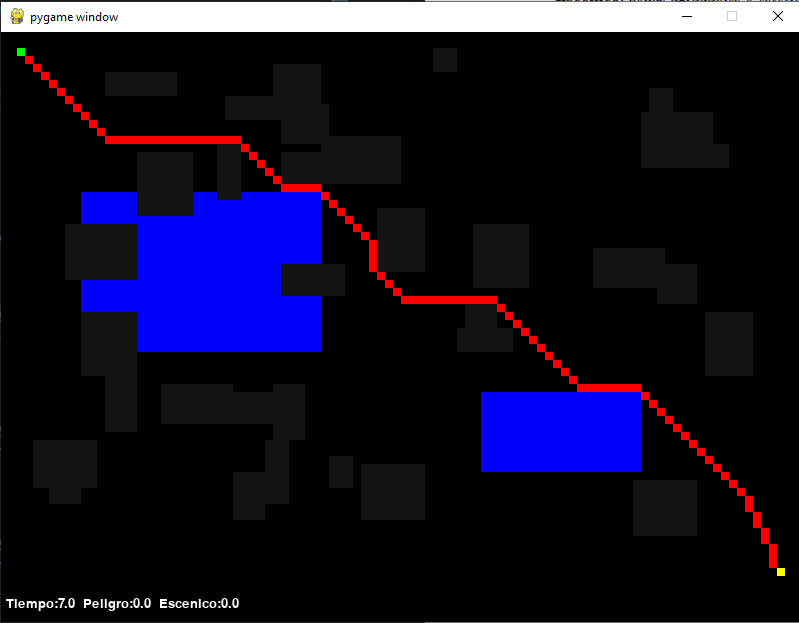
\includegraphics[width=0.85\textwidth]{ruta_tiempo_alto.PNG}
    \caption{Ruta con peso de tiempo alto (\(w_t\) grande). La ruta evita zonas azules lentas.}
\end{figure}

\begin{figure}[H]
    \centering
    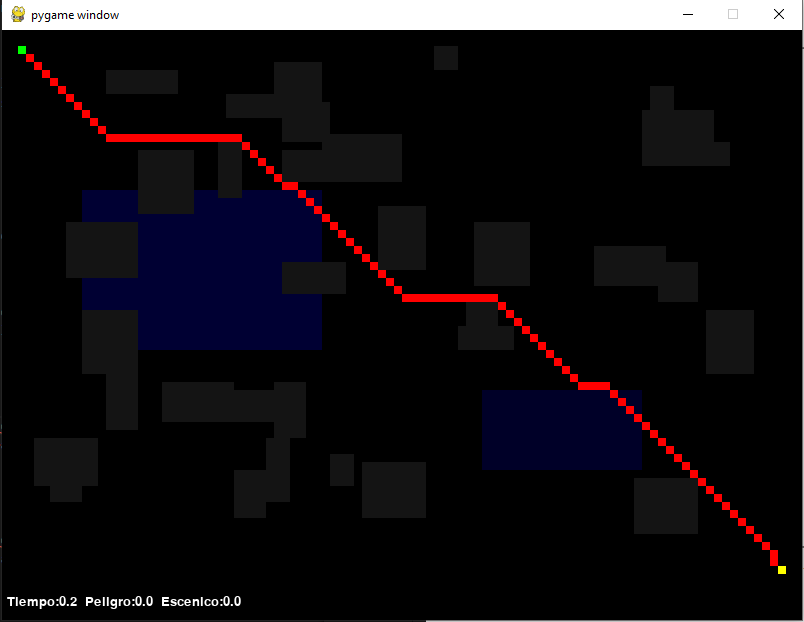
\includegraphics[width=0.85\textwidth]{ruta_tiempo_bajo.png}
    \caption{Ruta con peso de tiempo bajo. El agente atraviesa zonas lentas.}
\end{figure}

\begin{figure}[H]
    \centering
    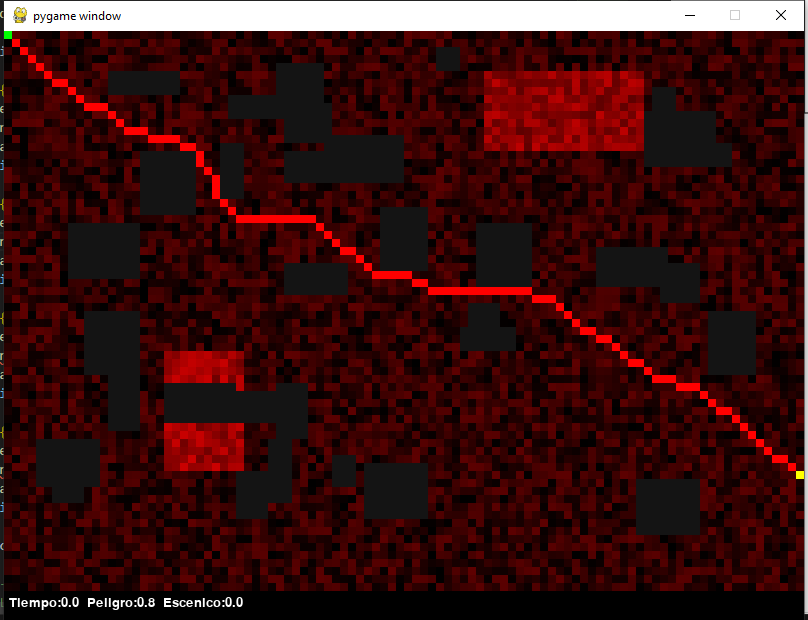
\includegraphics[width=0.85\textwidth]{ruta_peligro_alto.png}
    \caption{Ruta con peso de peligro alto. La trayectoria evita zonas rojas.}
\end{figure}

\begin{figure}[H]
    \centering
    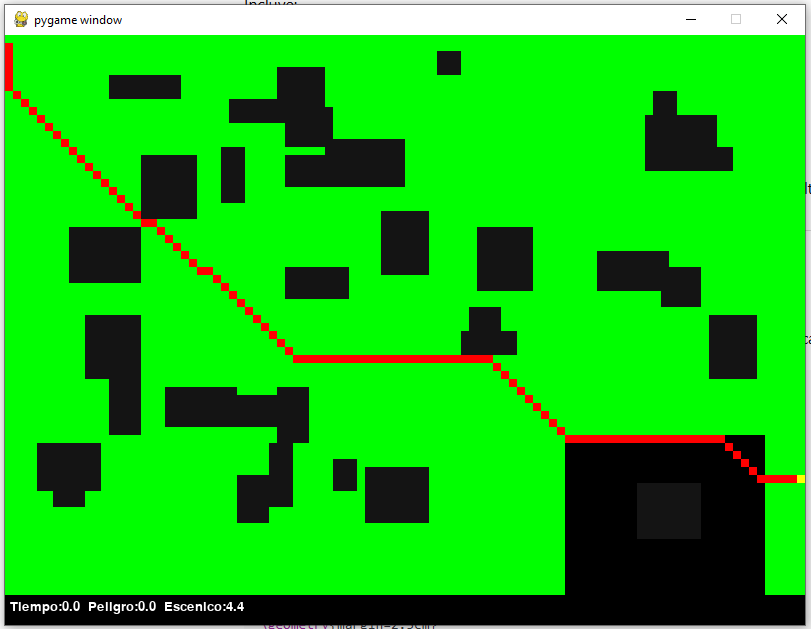
\includegraphics[width=0.85\textwidth]{ruta_escenico_alto.png}
    \caption{Ruta con peso escénico alto. Se favorecen las zonas verdes agradables.}
\end{figure}

Estas capturas demuestran cómo el algoritmo A* combina múltiples criterios para producir rutas óptimas de acuerdo con los valores establecidos por el usuario.

%--------------------------------------------------
% CONCLUSIONES
%--------------------------------------------------
\section{Conclusiones}

El experimento permitió observar de manera visual e interactiva cómo el algoritmo A* puede adaptarse a entornos complejos con múltiples factores de costo.

Se comprobó que:
\begin{itemize}
    \item Aumentar el peso de un criterio influye directamente en el trayecto seleccionado.
    \item La combinación ponderada de costos genera comportamientos realistas y ajustables.
    \item El uso de pygame facilita la comprensión intuitiva del funcionamiento de A* en entornos dinámicos.
\end{itemize}

En síntesis, la versión interactiva demuestra cómo la búsqueda informada puede extenderse más allá de la simple distancia, incorporando criterios contextuales como seguridad, velocidad o preferencia estética.

\vfill
\begin{center}
\textit{Fin del documento.}
\end{center}

\end{document}
